\thispagestyle{fancy}
\vspace*{40 pt}
\subsection{Tela de comando Alimentação} \label{sec:telaComandoAlimentacao}
Esta tela é acessada pelo botão "\textgreater" no menu superior esquerdo da tela de comando de máquina, pelo botão "\textless{}" no menu superior esquerdo da tela comando impressoras ou impressora 1, pelo botão \("\)ALM" em qualquer tela de comando e pelo botão comando da tela ajustes alimentação. A partir desta os botões "comando" e "ajustes" começam a se comportar de maneira contextual de maneira que eles vão levar a tela correspondente a tela selecionada. Caso você já esteja na tela selecionada você será levado a tela anterior.
\vspace*{\fill}
\begin{figure}[h]
    \centering
    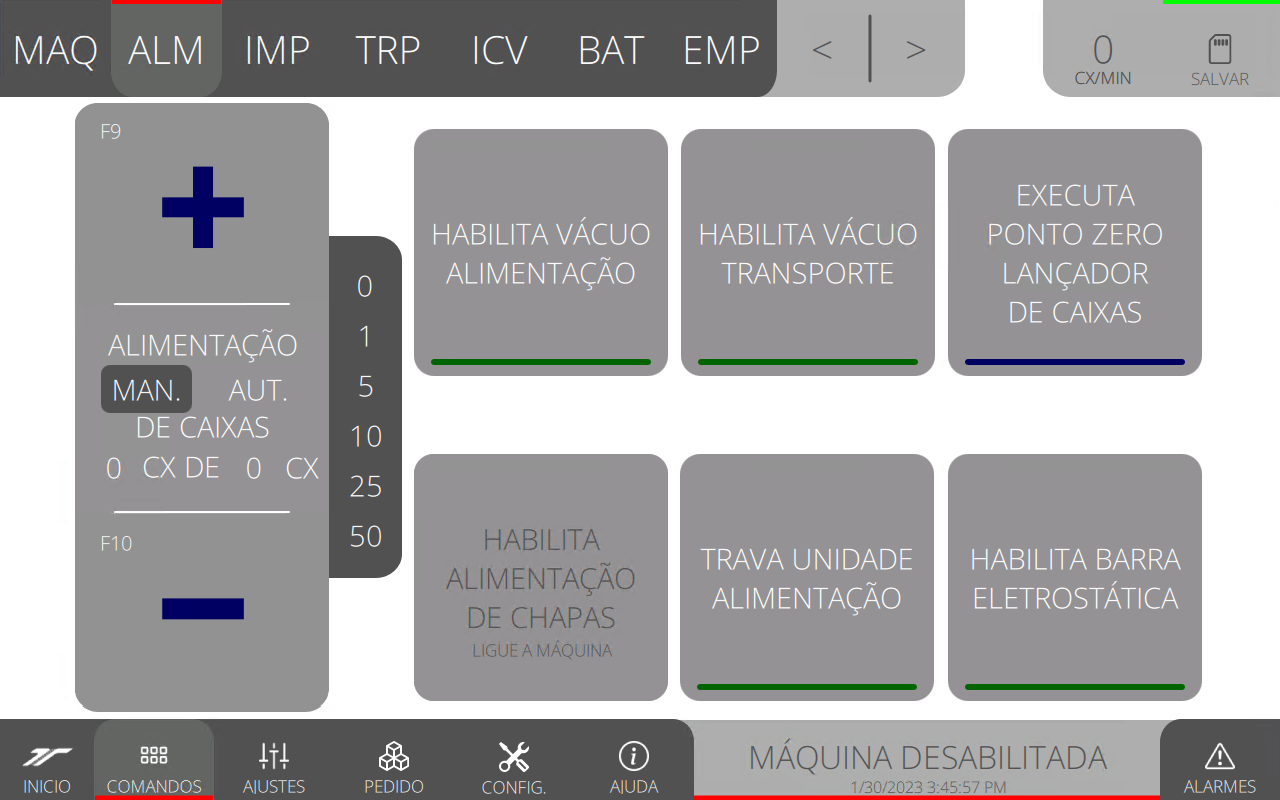
\includegraphics[width=480 px,height=300 px]{src/imagesICV/03-feeder/commands/1.png}
\end{figure}
\vspace*{\fill}

\newpage
\thispagestyle{fancy}
\vspace*{40 pt}
\subsubsection{\small{Alimentação manual da máquina}} \label{sec:telaComandoAlimentacaoAlimentacaoManualDaMaquina}
\vspace*{\fill}
\begin{figure}[h]
    \centering
    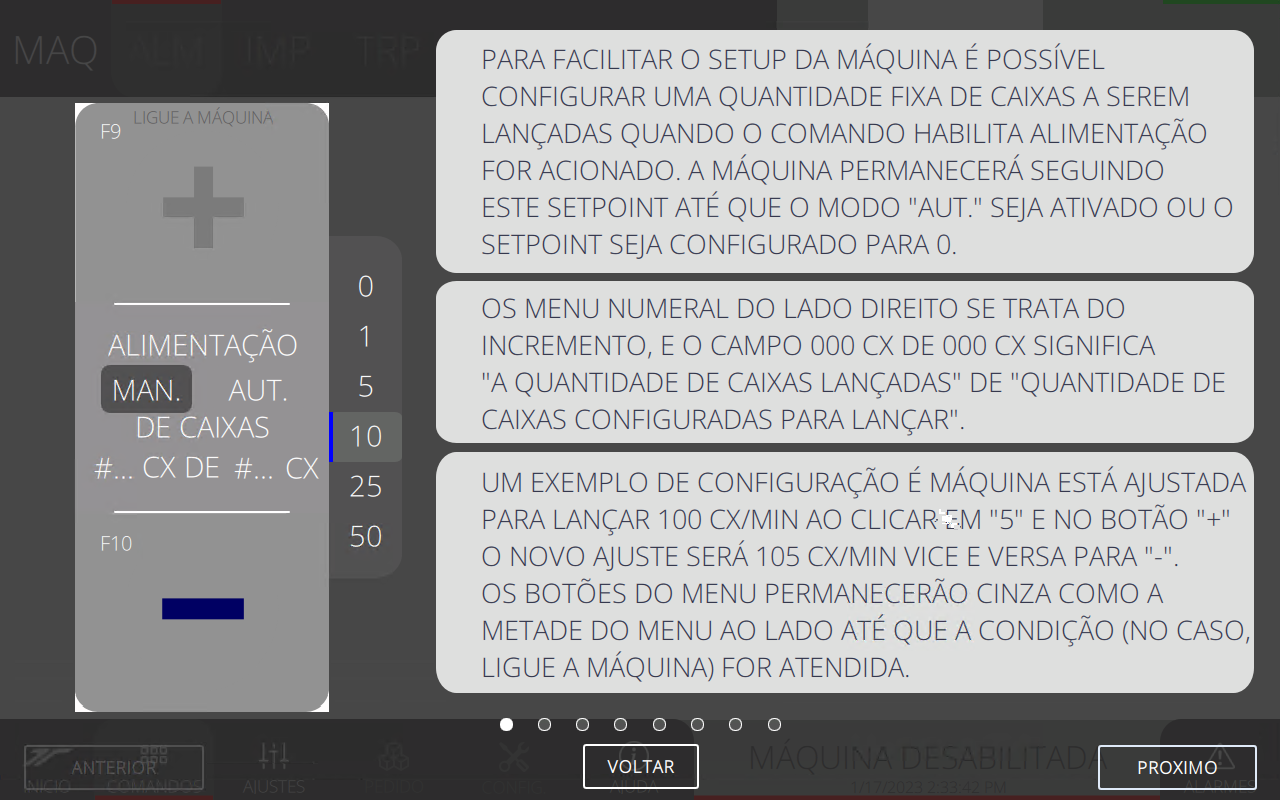
\includegraphics[width=576 px,height=360 px]{src/imagesICV/03-feeder/commands/2.png}
\end{figure}
\vspace*{\fill}

\newpage
\thispagestyle{fancy}
\vspace*{40 pt}
\subsubsection{\small{Alimentação automática da máquina}} \label{sec:telaComandoAlimentacaoAlimentacaoAutomaticaDaMaquina}
\vspace*{\fill}
\begin{figure}[h]
    \centering
    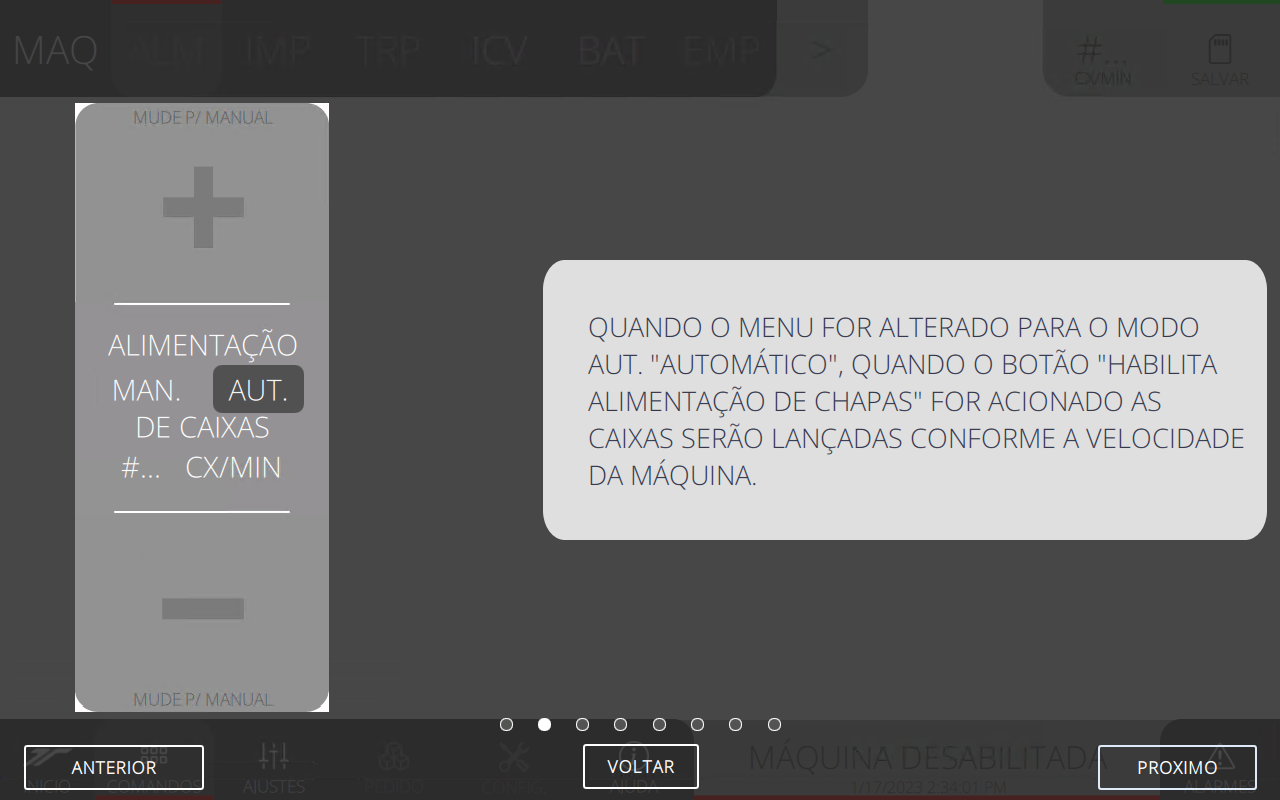
\includegraphics[width=576 px,height=360 px]{src/imagesICV/03-feeder/commands/3.png}
\end{figure}
\vspace*{\fill}

\newpage
\thispagestyle{fancy}
\vspace*{40 pt}
\subsubsection{\small{Habilita vácuo transporte}} \label{sec:telaComandoAlimentacaoHabilitaVacoTransporte}
\vspace*{\fill}
\begin{figure}[h]
    \centering
    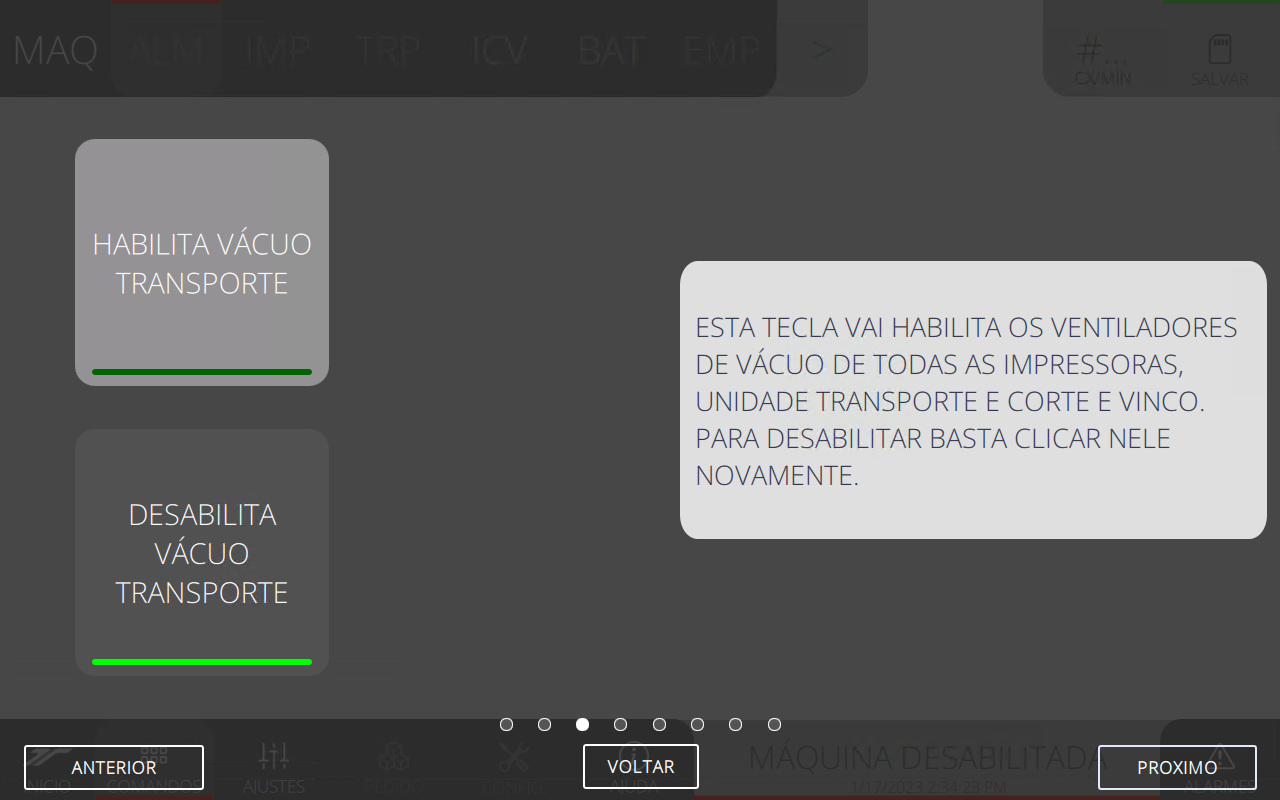
\includegraphics[width=576 px,height=360 px]{src/imagesICV/03-feeder/commands/4.png}
\end{figure}
\vspace*{\fill}

\newpage
\thispagestyle{fancy}
\vspace*{40 pt}
\subsubsection{\small{Habilita vácuo alimentação}} \label{sec:telaComandoAlimentacaoHabilitaVacoAlimentacao}
\vspace*{\fill}
\begin{figure}[h]
    \centering
    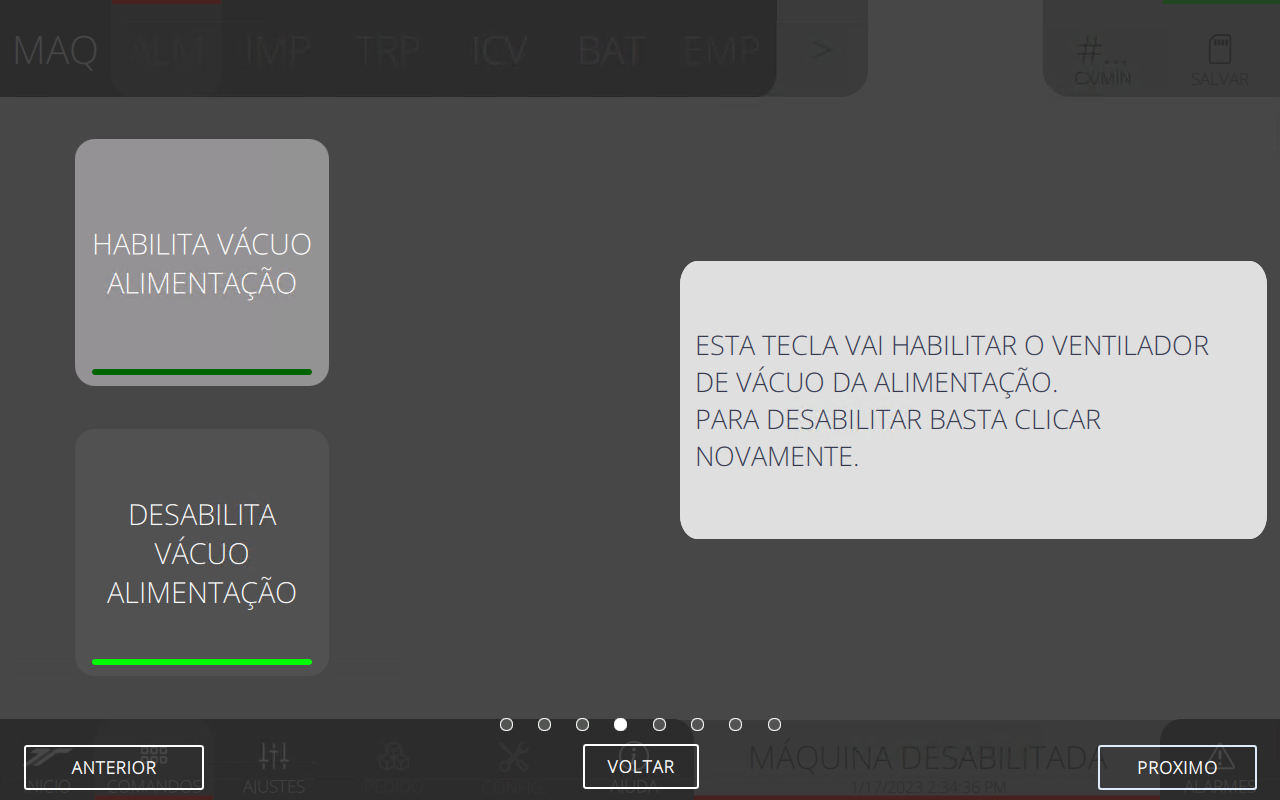
\includegraphics[width=576 px,height=360 px]{src/imagesICV/03-feeder/commands/5.png}
\end{figure}
\vspace*{\fill}

\newpage
\thispagestyle{fancy}
\vspace*{40 pt}
\subsubsection{\small{Executa ponto zero Lançador de Caixas}} \label{sec:telaComandoAlimentacaoExecutaPontoZeroLancadorDeCaixas}
\vspace*{\fill}
\begin{figure}[h]
    \centering
    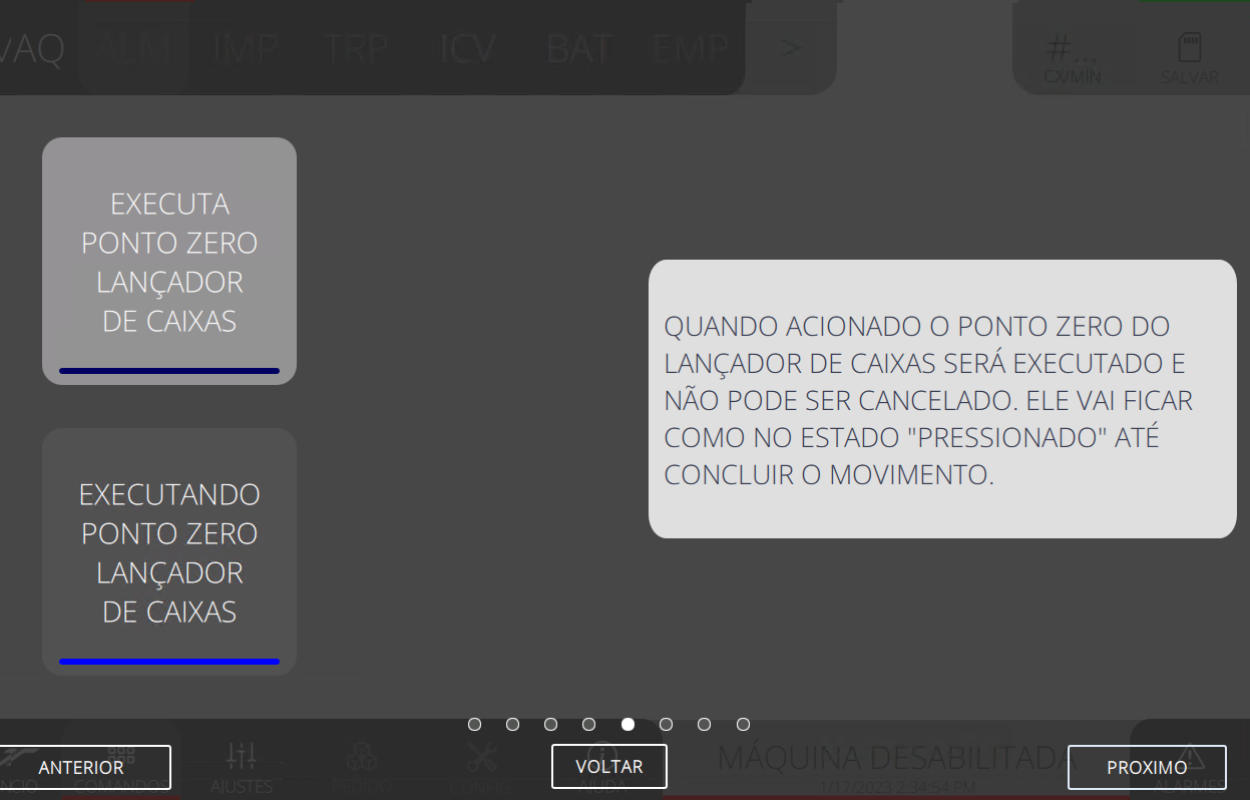
\includegraphics[width=576 px,height=360 px]{src/imagesICV/03-feeder/commands/6.png}
\end{figure}
\vspace*{\fill}

\newpage
\thispagestyle{fancy}
\vspace*{40 pt}
\subsubsection{\small{Habilita alimentação de chapas}} \label{sec:telaComandoAlimentacaoHabilitaAlimentacaoDeChapas}
\vspace*{\fill}
\begin{figure}[h]
    \centering
    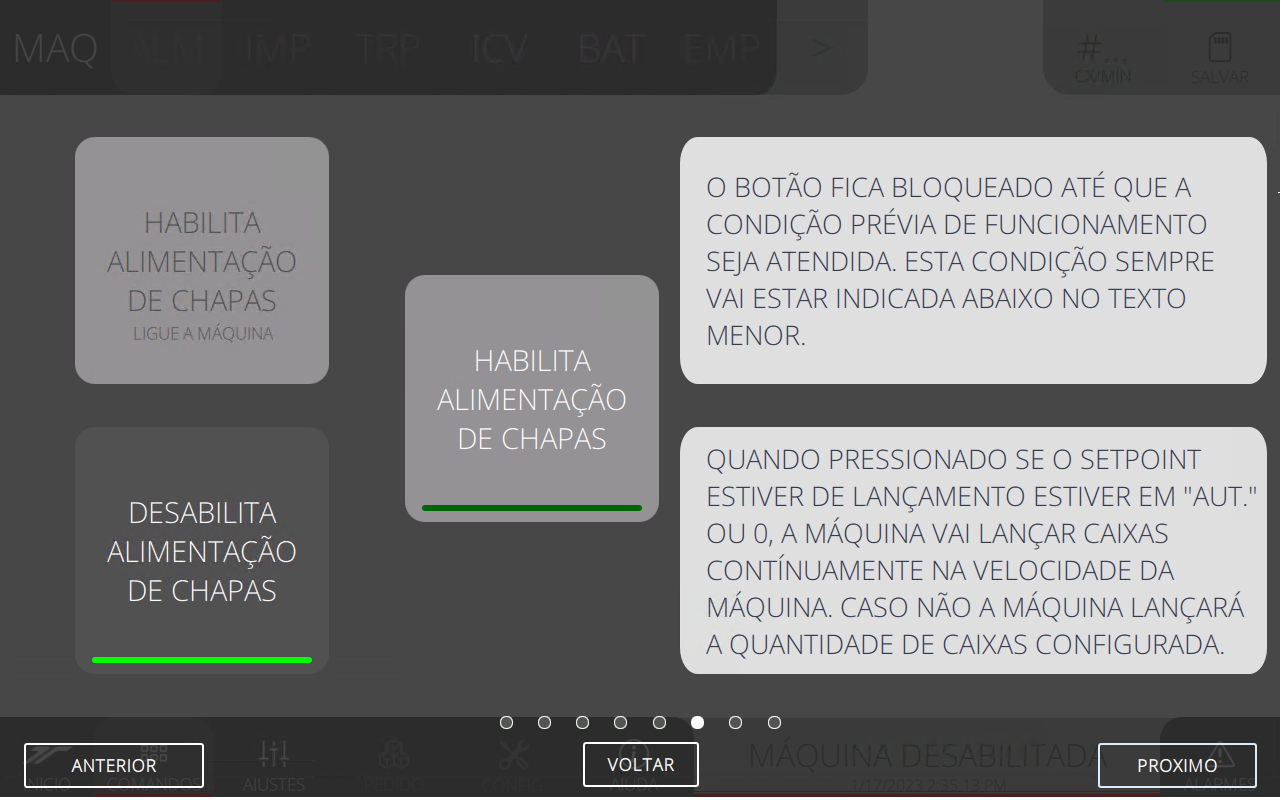
\includegraphics[width=576 px,height=360 px]{src/imagesICV/03-feeder/commands/7.png}
\end{figure}
\vspace*{\fill}

\newpage
\thispagestyle{fancy}
\vspace*{40 pt}
\subsubsection{\small{Trava unidade alimentação}} \label{sec:telaComandoAlimentacaoTravaUnidadeAlimentacao}
\vspace*{\fill}
\begin{figure}[h]
    \centering
    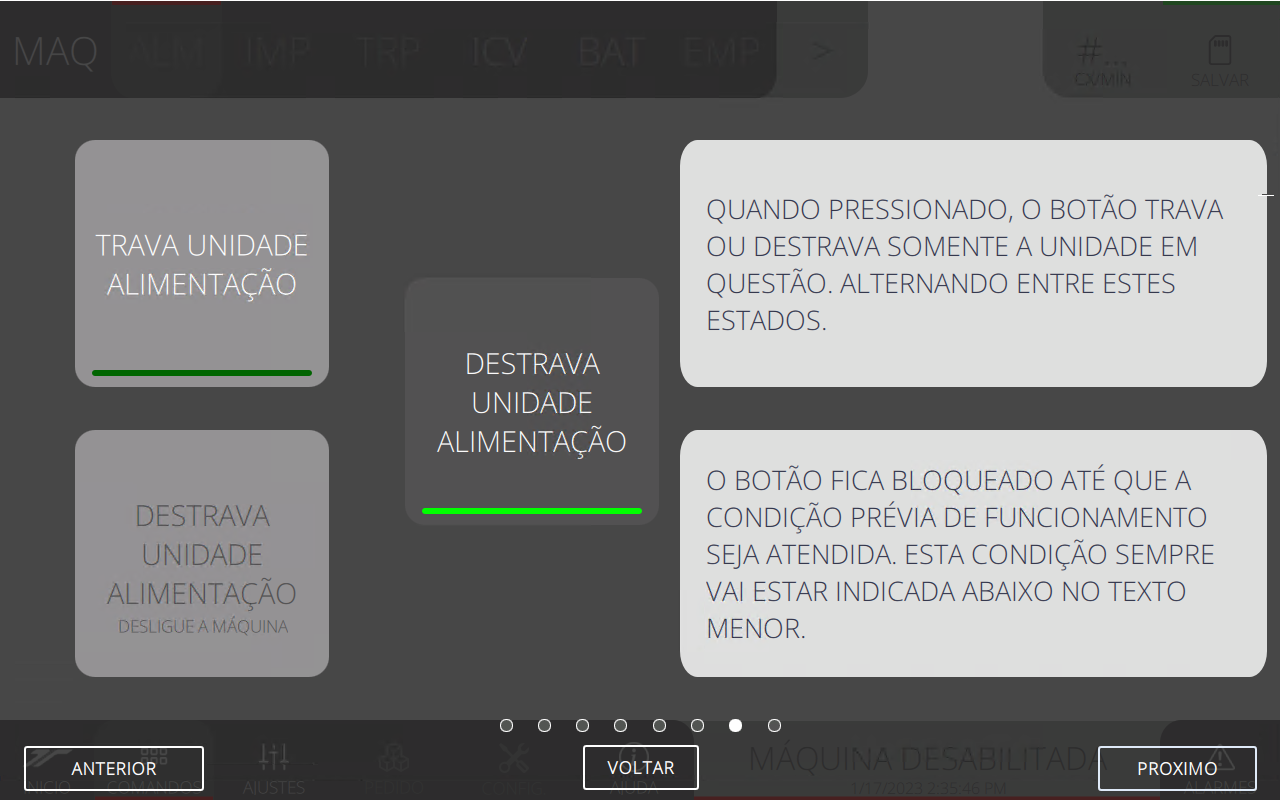
\includegraphics[width=576 px,height=360 px]{src/imagesICV/03-feeder/commands/8.png}
\end{figure}
\vspace*{\fill}

\newpage
\thispagestyle{fancy}
\vspace*{40 pt}
\subsubsection{\small{Habilita barra eletrostática}} \label{sec:telaComandoAlimentacaoHabilitaBarraEletrosttica}
\vspace*{\fill}
\begin{figure}[h]
    \centering
    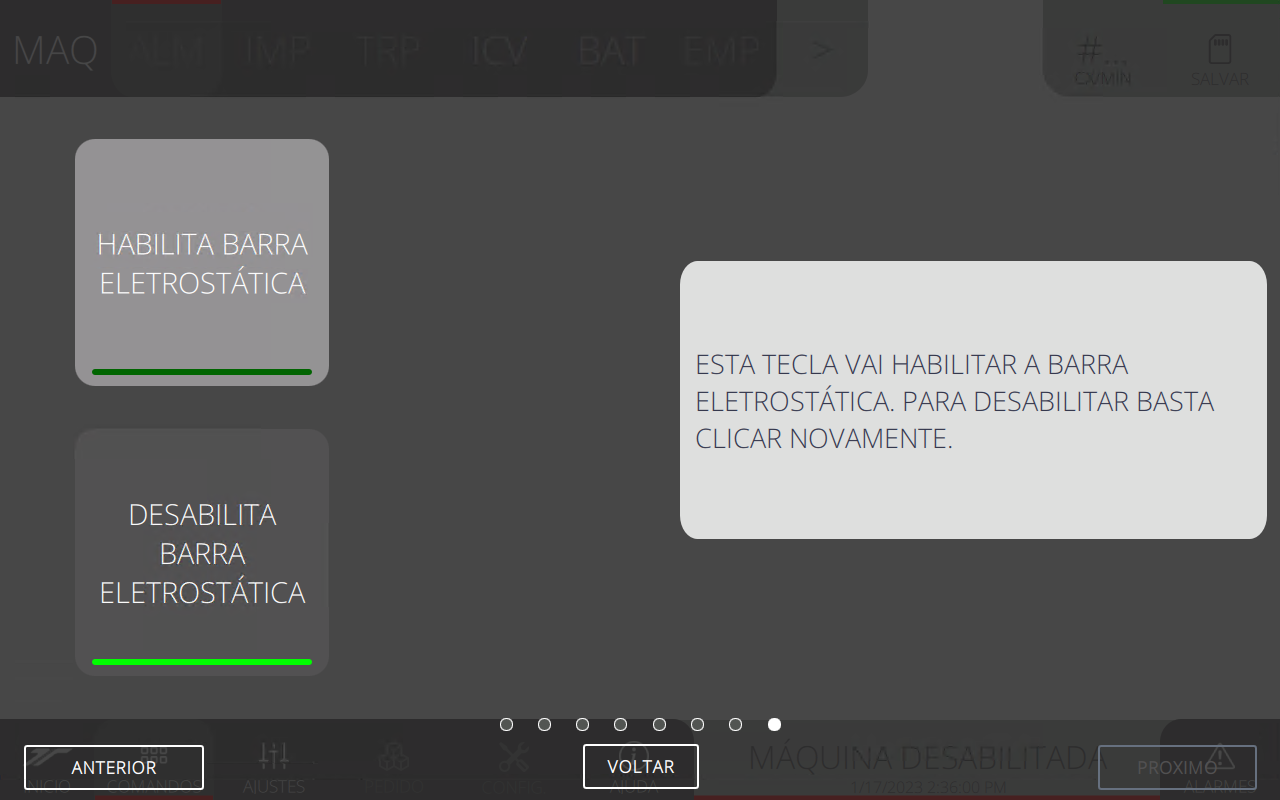
\includegraphics[width=576 px,height=360 px]{src/imagesICV/03-feeder/commands/9.png}
\end{figure}
\vspace*{\fill}